\documentclass{standalone}
\usepackage{tikz}
\usetikzlibrary{patterns, positioning}

\begin{document}
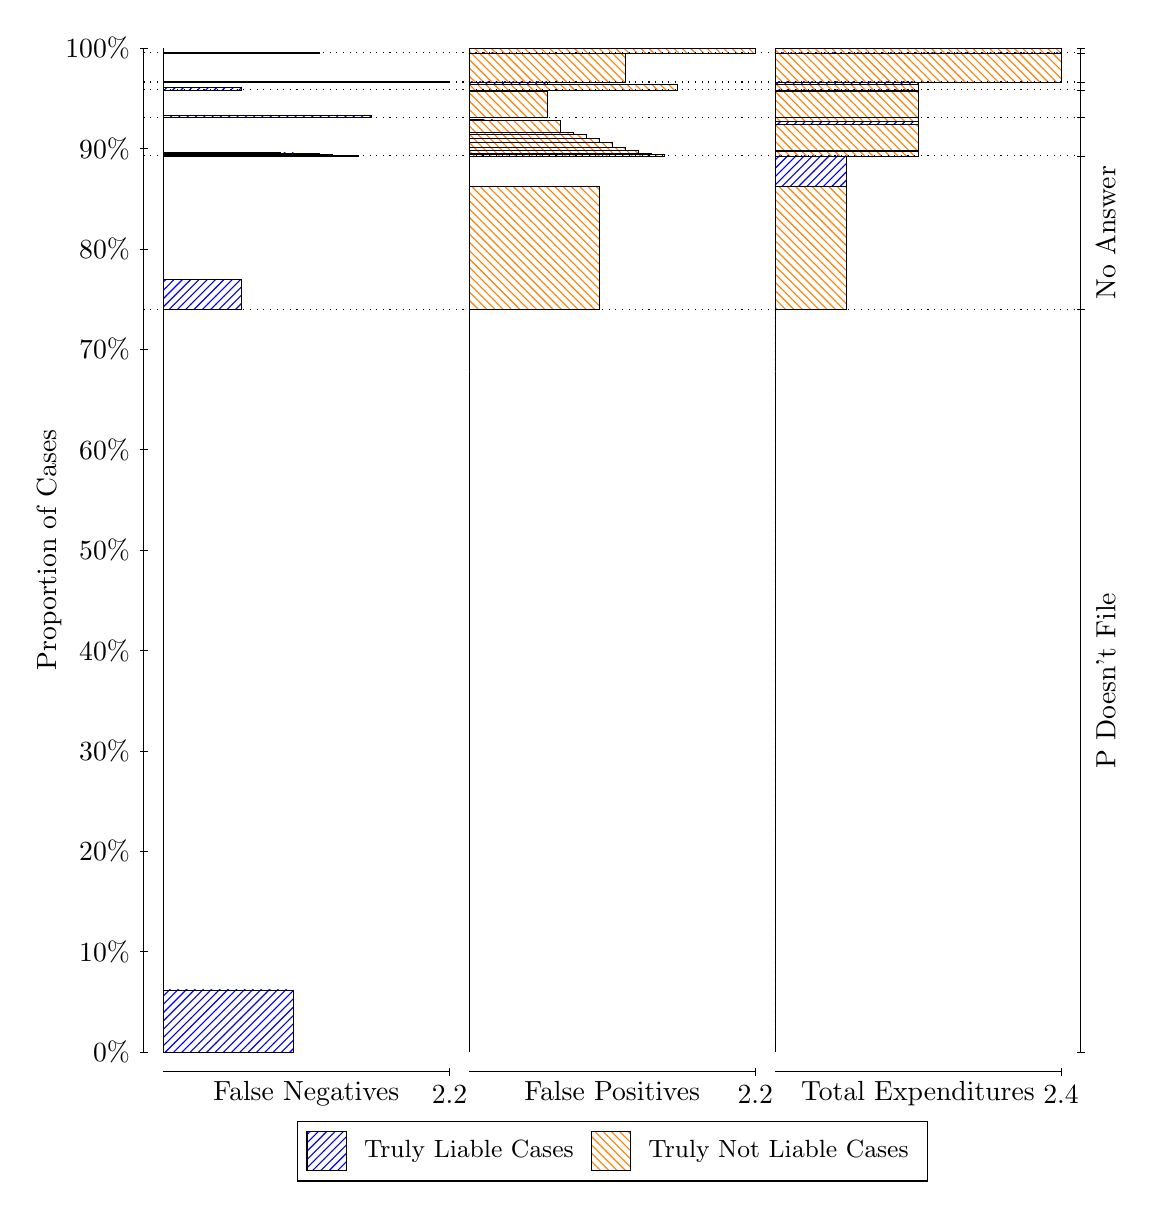
\begin{tikzpicture}
\draw[black, very thin] (1.5,1.75) -- (1.5,14.5);
\node[rotate=90, anchor=center] at (0.3, 8.125) {Proportion of Cases};
\draw[black, very thin] (1.45,1.75) -- (1.55,1.75);
\node[anchor=east] at (1.45, 1.75) {0\%};
\draw[black, very thin] (1.45,3.025) -- (1.55,3.025);
\node[anchor=east] at (1.45, 3.025) {10\%};
\draw[black, very thin] (1.45,4.3) -- (1.55,4.3);
\node[anchor=east] at (1.45, 4.3) {20\%};
\draw[black, very thin] (1.45,5.575) -- (1.55,5.575);
\node[anchor=east] at (1.45, 5.575) {30\%};
\draw[black, very thin] (1.45,6.85) -- (1.55,6.85);
\node[anchor=east] at (1.45, 6.85) {40\%};
\draw[black, very thin] (1.45,8.125) -- (1.55,8.125);
\node[anchor=east] at (1.45, 8.125) {50\%};
\draw[black, very thin] (1.45,9.4) -- (1.55,9.4);
\node[anchor=east] at (1.45, 9.4) {60\%};
\draw[black, very thin] (1.45,10.675) -- (1.55,10.675);
\node[anchor=east] at (1.45, 10.675) {70\%};
\draw[black, very thin] (1.45,11.95) -- (1.55,11.95);
\node[anchor=east] at (1.45, 11.95) {80\%};
\draw[black, very thin] (1.45,13.225) -- (1.55,13.225);
\node[anchor=east] at (1.45, 13.225) {90\%};
\draw[black, very thin] (1.45,14.5) -- (1.55,14.5);
\node[anchor=east] at (1.45, 14.5) {100\%};

\draw[black, very thin] (13.4,1.75) -- (13.4,14.5);
\draw[black, very thin] (13.35,1.75) -- (13.45,1.75);
\node[anchor=west] at (13.35, 1.75) {};
\draw[black, very thin] (13.35,11.179) -- (13.45,11.179);
\node[anchor=west] at (13.35, 11.179) {};
\draw[black, very thin] (13.35,13.13) -- (13.45,13.13);
\node[anchor=west] at (13.35, 13.13) {};
\draw[black, very thin] (13.35,13.622) -- (13.45,13.622);
\node[anchor=west] at (13.35, 13.622) {};
\draw[black, very thin] (13.35,13.969) -- (13.45,13.969);
\node[anchor=west] at (13.35, 13.969) {};
\draw[black, very thin] (13.35,14.069) -- (13.45,14.069);
\node[anchor=west] at (13.35, 14.069) {};
\draw[black, very thin] (13.35,14.439) -- (13.45,14.439);
\node[anchor=west] at (13.35, 14.439) {};
\draw[black, very thin] (13.35,14.5) -- (13.45,14.5);
\node[anchor=west] at (13.35, 14.5) {};

\draw[black, very thin, pattern color=blue, pattern=north east lines] (1.75,1.75) rectangle (3.4015,2.538);
\draw[black, very thin, pattern color=orange, pattern=north west lines] (1.75,2.538) rectangle (1.75,11.179);
\draw[black, very thin, pattern color=blue, pattern=north east lines] (1.75,11.179) rectangle (2.7409,11.562);
\draw[black, very thin, pattern color=orange, pattern=north west lines] (1.75,11.562) rectangle (1.75,13.13);
\draw[black, very thin, pattern color=blue, pattern=north east lines] (1.75,13.13) rectangle (4.2273,13.136);
\draw[black, very thin, pattern color=blue, pattern=north east lines] (1.75,13.136) rectangle (4.0621,13.14);
\draw[black, very thin, pattern color=blue, pattern=north east lines] (1.75,13.14) rectangle (3.897,13.152);
\draw[black, very thin, pattern color=blue, pattern=north east lines] (1.75,13.152) rectangle (3.7318,13.158);
\draw[black, very thin, pattern color=blue, pattern=north east lines] (1.75,13.158) rectangle (3.5667,13.165);
\draw[black, very thin, pattern color=blue, pattern=north east lines] (1.75,13.165) rectangle (3.4015,13.169);
\draw[black, very thin, pattern color=blue, pattern=north east lines] (1.75,13.169) rectangle (3.2364,13.172);
\draw[black, very thin, pattern color=blue, pattern=north east lines] (1.75,13.172) rectangle (3.0712,13.174);
\draw[black, very thin, pattern color=blue, pattern=north east lines] (1.75,13.174) rectangle (2.9061,13.175);
\draw[black, very thin, pattern color=orange, pattern=north west lines] (1.75,13.175) rectangle (1.75,13.622);
\draw[black, very thin, pattern color=blue, pattern=north east lines] (1.75,13.622) rectangle (4.3924,13.641);
\draw[black, very thin, pattern color=orange, pattern=north west lines] (1.75,13.641) rectangle (1.75,13.969);
\draw[black, very thin, pattern color=blue, pattern=north east lines] (1.75,13.969) rectangle (2.7409,13.996);
\draw[black, very thin, pattern color=orange, pattern=north west lines] (1.75,13.996) rectangle (1.75,14.069);
\draw[black, very thin, pattern color=blue, pattern=north east lines] (1.75,14.069) rectangle (5.3833,14.075);
\draw[black, very thin, pattern color=orange, pattern=north west lines] (1.75,14.075) rectangle (1.75,14.439);
\draw[black, very thin, pattern color=blue, pattern=north east lines] (1.75,14.439) rectangle (3.7318,14.446);
\draw[black, very thin, pattern color=orange, pattern=north west lines] (1.75,14.446) rectangle (1.75,14.5);
\draw[black, very thin, pattern color=orange, pattern=north west lines] (5.6333,1.75) rectangle (5.6333,10.391);
\draw[black, very thin, pattern color=blue, pattern=north east lines] (5.6333,10.391) rectangle (5.6333,11.179);
\draw[black, very thin, pattern color=orange, pattern=north west lines] (5.6333,11.179) rectangle (7.2848,12.747);
\draw[black, very thin, pattern color=blue, pattern=north east lines] (5.6333,12.747) rectangle (5.6333,13.13);
\draw[black, very thin, pattern color=orange, pattern=north west lines] (5.6333,13.13) rectangle (8.1106,13.146);
\draw[black, very thin, pattern color=orange, pattern=north west lines] (5.6333,13.146) rectangle (7.9455,13.163);
\draw[black, very thin, pattern color=orange, pattern=north west lines] (5.6333,13.163) rectangle (7.7803,13.197);
\draw[black, very thin, pattern color=orange, pattern=north west lines] (5.6333,13.197) rectangle (7.6152,13.243);
\draw[black, very thin, pattern color=orange, pattern=north west lines] (5.6333,13.243) rectangle (7.45,13.306);
\draw[black, very thin, pattern color=orange, pattern=north west lines] (5.6333,13.306) rectangle (7.2848,13.353);
\draw[black, very thin, pattern color=orange, pattern=north west lines] (5.6333,13.353) rectangle (7.1197,13.405);
\draw[black, very thin, pattern color=orange, pattern=north west lines] (5.6333,13.405) rectangle (6.9545,13.425);
\draw[black, very thin, pattern color=orange, pattern=north west lines] (5.6333,13.425) rectangle (6.7894,13.578);
\draw[black, very thin, pattern color=blue, pattern=north east lines] (5.6333,13.578) rectangle (6.4591,13.579);
\draw[black, very thin, pattern color=blue, pattern=north east lines] (5.6333,13.579) rectangle (6.2939,13.58);
\draw[black, very thin, pattern color=blue, pattern=north east lines] (5.6333,13.58) rectangle (6.1288,13.584);
\draw[black, very thin, pattern color=blue, pattern=north east lines] (5.6333,13.584) rectangle (5.9636,13.588);
\draw[black, very thin, pattern color=blue, pattern=north east lines] (5.6333,13.588) rectangle (5.7985,13.595);
\draw[black, very thin, pattern color=blue, pattern=north east lines] (5.6333,13.595) rectangle (5.6333,13.622);
\draw[black, very thin, pattern color=orange, pattern=north west lines] (5.6333,13.622) rectangle (6.6242,13.951);
\draw[black, very thin, pattern color=blue, pattern=north east lines] (5.6333,13.951) rectangle (5.6333,13.969);
\draw[black, very thin, pattern color=orange, pattern=north west lines] (5.6333,13.969) rectangle (8.2758,14.042);
\draw[black, very thin, pattern color=blue, pattern=north east lines] (5.6333,14.042) rectangle (6.6242,14.069);
\draw[black, very thin, pattern color=orange, pattern=north west lines] (5.6333,14.069) rectangle (7.6152,14.433);
\draw[black, very thin, pattern color=blue, pattern=north east lines] (5.6333,14.433) rectangle (5.9636,14.439);
\draw[black, very thin, pattern color=orange, pattern=north west lines] (5.6333,14.439) rectangle (9.2667,14.492);
\draw[black, very thin, pattern color=blue, pattern=north east lines] (5.6333,14.492) rectangle (7.6152,14.5);
\draw[black, very thin, pattern color=orange, pattern=north west lines] (9.5167,1.75) rectangle (9.5167,10.391);
\draw[black, very thin, pattern color=blue, pattern=north east lines] (9.5167,10.391) rectangle (9.5167,11.179);
\draw[black, very thin, pattern color=orange, pattern=north west lines] (9.5167,11.179) rectangle (10.425,12.747);
\draw[black, very thin, pattern color=blue, pattern=north east lines] (9.5167,12.747) rectangle (10.425,13.13);
\draw[black, very thin, pattern color=orange, pattern=north west lines] (9.5167,13.13) rectangle (11.333,13.194);
\draw[black, very thin, pattern color=blue, pattern=north east lines] (9.5167,13.194) rectangle (11.333,13.201);
\draw[black, very thin, pattern color=orange, pattern=north west lines] (9.5167,13.201) rectangle (11.333,13.534);
\draw[black, very thin, pattern color=blue, pattern=north east lines] (9.5167,13.534) rectangle (11.333,13.567);
\draw[black, very thin, pattern color=orange, pattern=north west lines] (9.5167,13.567) rectangle (11.333,13.618);
\draw[black, very thin, pattern color=blue, pattern=north east lines] (9.5167,13.618) rectangle (11.333,13.622);
\draw[black, very thin, pattern color=orange, pattern=north west lines] (9.5167,13.622) rectangle (11.333,13.951);
\draw[black, very thin, pattern color=blue, pattern=north east lines] (9.5167,13.951) rectangle (11.333,13.969);
\draw[black, very thin, pattern color=orange, pattern=north west lines] (9.5167,13.969) rectangle (11.333,14.042);
\draw[black, very thin, pattern color=blue, pattern=north east lines] (9.5167,14.042) rectangle (11.333,14.069);
\draw[black, very thin, pattern color=orange, pattern=north west lines] (9.5167,14.069) rectangle (13.15,14.433);
\draw[black, very thin, pattern color=blue, pattern=north east lines] (9.5167,14.433) rectangle (13.15,14.439);
\draw[black, very thin, pattern color=orange, pattern=north west lines] (9.5167,14.439) rectangle (13.15,14.492);
\draw[black, very thin, pattern color=blue, pattern=north east lines] (9.5167,14.492) rectangle (13.15,14.5);
\draw[black, dotted] (1.5,11.179) -- (13.4,11.179);
\draw[black, dotted] (1.5,13.13) -- (13.4,13.13);
\draw[black, dotted] (1.5,13.622) -- (13.4,13.622);
\draw[black, dotted] (1.5,13.969) -- (13.4,13.969);
\draw[black, dotted] (1.5,14.069) -- (13.4,14.069);
\draw[black, dotted] (1.5,14.439) -- (13.4,14.439);
\draw[black, very thin] (1.75,1.5) -- (5.3833,1.5);
\node[anchor=north] at (3.5667, 1.5) {False Negatives};
\draw[black, very thin] (5.3833,1.45) -- (5.3833,1.55);
\node[anchor=north] at (5.3833, 1.45) {2.2};

\draw[black, very thin] (5.6333,1.5) -- (9.2667,1.5);
\node[anchor=north] at (7.45, 1.5) {False Positives};
\draw[black, very thin] (9.2667,1.45) -- (9.2667,1.55);
\node[anchor=north] at (9.2667, 1.45) {2.2};

\draw[black, very thin] (9.5167,1.5) -- (13.15,1.5);
\node[anchor=north] at (11.333, 1.5) {Total Expenditures};
\draw[black, very thin] (13.15,1.45) -- (13.15,1.55);
\node[anchor=north] at (13.15, 1.45) {2.4};

\node[black, centered, rotate=90] at (13.72, 6.4644) {P Doesn't File};
\node[black, centered, rotate=90] at (13.72, 12.154) {No Answer};






\draw (7.449999999999999,1.5) node[draw=none] (baseCoordinate) {};
\begin{scope}[align=center]
        \matrix[scale=0.5, draw=black, below=0.5cm of baseCoordinate, nodes={draw}, column sep=0.1cm]{
            \node[rectangle, draw, minimum width=0.5cm, minimum height=0.5cm, pattern=north east lines, pattern color=blue] {}; &
            \node[draw=none, font=\small] (B) {Truly Liable Cases}; &
            \node[rectangle, draw, minimum width=0.5cm, minimum height=0.5cm, pattern=north west lines, pattern color=orange] {}; &
            \node[draw=none, font=\small] (B) {Truly Not Liable Cases}; \\
            };
\end{scope}

\end{tikzpicture}
\end{document}